\chapter{YOLO}
\ac{yolo} ist ein populäres Objekt Erkennungsmodell, dass dafür bekannt ist besonders schnell und akkurat Objekte in Bildern zu erkennen. Dies liegt an der kleinen Modellgröße und den hohen Berechnungsgeschwindigkeiten. Des Weiteren nutzt \ac{yolo} das gesamte Bild als Trainingsgrundlage, was es sowohl ermöglicht Videos zu klassifizieren als auch die Fehlerrate reduziert, dass der Hintergrund als Teil des Objektes klassifiziert wird. In diesem Kapitel geht es darum wie die Schnittstelle bzw. der Algorithmus gefüttert werden muss und was der Algorithmus für Datenformate erwartet \cite{Jiang.2022}.

\begin{wrapfigure}{r}{5cm}
    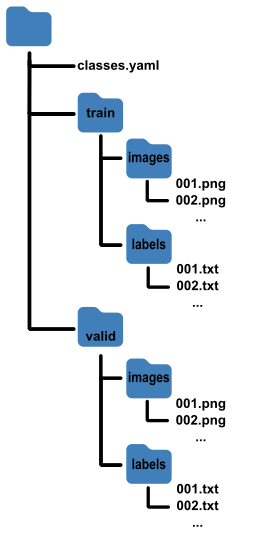
\includegraphics[width=5cm]{data/img/ordnerstruktur_yolo.png}
    \caption*{Ordnerstruktur für einen Datensatz}
    \label{fig:folderYolo}
\end{wrapfigure}

Für die Studienarbeit wird der YOLOv5 von ultralytics \cite{glennjocher.2023} genommenm, da diese folgende Vorteile bietet:
\begin{itemize}
    \item aktive Developer am Projekt
    \item große Community 
    \item Docker deployable
    \item CUDA- und GPU-Unterstützung
    \item Pytorch Beschleungigung
\end{itemize}


\section*{Generelle Ordnerstruktur}
Der \ac{yolo}-Algorithmus erwartet zum funktionieren eine generelle Ordnerstruktur, gezeigt in \ref{fig:folderYolo}. Der oberste Ordner ist dabei der Projektnameordner. In diesem müssen alle Projektrelevanten Bilder und Label enthalten sein. 

Auch darin enthalten sein muss das \textit{.yaml} file. Das wird in Kapitel \ref{sec:yaml_class} noch mal genauer beschrieben. Ansonsten müssen neben dem \textit{.yaml} file noch ein Ordner für die Trainingsdaten enthalten sein. Optional auch ein Testdatenordner und Validierungsdatenordner.

\section*{YAML Klassifizierungsfile}
\label{sec:yaml_class}
